\chapter{Experiments} \label{chp:experiments}
\section{Suppression Task} \label{sec:sup}
\subsection{Intuitive Overview} \label{ssec:sup_intuition}
The Suppression Task refers to an experiment conducted by \cite{byrne1989suppressing} and is a classical example of the inadequacy of monotonic logics for modelling human reasoning. In classical logic, if our knowledge base $kb$ is such that $kb \models \phi$, then it must be the case that $kb \cup \psi \models \phi$. However, in the suppression task participants no longer draw classically valid inferences when new information is added. The task is often formulated as follows:

\begin{itemize}
\item $e \rightarrow l$: If she has an essay to write ($e$), she will study late in the library ($l$).
\item $\top \rightarrow e$: She has an essay to write ($e$).
\item $o\rightarrow l$: If the library is open ($o$), she will study late in the library ($l$).
\end{itemize}

Given only the rules $(e \rightarrow l)$ and $(\top \rightarrow e)$, the participants consistently concluded that she would study late in the library, seemingly drawing the classical logic inference $\frac{e \rightarrow l, e}{l}$ with \textit{modus ponens}. But when given the additional rule $o\rightarrow l$, participants no longer believe that they have enough information to judge whether she will study late in the library, and a significant portion of them no longer draw the classical conclusion. This effect, called Suppression, demonstrates the need for something more than classical logic for modelling human reasoning.

\subsection{Modelling the Suppression Task} \label{ssec:sup_mod}
Work by \cite{dietz2014modeling} has shown that the WCS is an adequate non-monotonic logic for modelling the Suppression Task. Under the WCS and \L ukasiewicz 3-valued logic the task is usually modelled as follows for the case without suppression:
\begin{enumerate}
\item $KB=(\{e \leftarrow \top\}, \Delta=\{(l|e)\})$
\item Initial logic program: $P = \{e \rightarrow l, \top \rightarrow e \}$. This program represents the task without information about what happens if the library is open.
\item Interpretation of conditionals: $P = \{e \land \lnot ab_1 \rightarrow l, \top \rightarrow e, \bot \rightarrow ab_1 \}$. Treating the conditional as a license for implication (Section~\ref{ssec:condInterpretation}). The program now reflects the possibility that some abnormal event may prevent her from going to the library, but because we have no information about the nature of this event, it is set to $\bot$ by default.
\item Weak Completion: $wc(P) = \{e \land \lnot ab_1 \leftrightarrow l, \top \leftrightarrow e, \bot \leftrightarrow ab_1 \}$.
\item Semantic Operator:
\begin{itemize}
\item Execution 1: $\top=\{e\}, \bot=\{ab_1\}$
\item Execution 2: $\top=\{e,l\}, \bot=\{ab_1\}$
\end{itemize}
\end{enumerate}

After application of the semantic operator $l$ is true in the least model, and so participants conclude that she will study late in the library (as when $P$ is evaluated classically). However, in the case where Suppression is observed, the same process yields a different result because of the presence of the extra conditional ($o\rightarrow l$).
\begin{enumerate}
\item Initial logic program: $P = \{e \rightarrow l, \top \rightarrow e, o \rightarrow l \}$. The initial program now includes information about the extra (suppressing) conditional.
\item Addition of Abnormality: $P = \{e \land \lnot ab_1 \rightarrow l, o \land \lnot ab_2 \rightarrow l, \top \rightarrow e, \lnot o \rightarrow ab_1, \lnot e \rightarrow ab_2 \}$. An abnormality $ab_i$ is an addition to an inference which captures the idea that external factors may invalidate the conclusion of the original inference. Adding abnormalities is a poorly described process and often relies on intuitionist views of what actually constitutes an abnormal situation.
\item Weak Completion: $wc(P) = \{((e \land \lnot ab_1) \lor (o \land \lnot ab_2)) \leftrightarrow l, \top \leftrightarrow e, \lnot o \leftrightarrow ab_1, \lnot e \leftrightarrow ab_2 \}$. Weak completion is applied to the logic program, combining rules with shared heads and replacing implications with bijections.
\item Semantic Operator:
\begin{itemize}
\item Execution 1: $\top=\{e\}, \bot=\{ab_2\}$
\end{itemize}
\end{enumerate}

Now suppression has been displayed in the logic program and the variable $l$ remains unknown in the least model.

@TODORefragnipaper showed that suppression is not possible in Reiter's default logic.

\section{Wason Selection Task}
\begin{table}
\begin{center}


\begin{tabular}{ c c c c c}
  & \textbf{$p$} & \textbf{$pq$} & \textbf{$pq\bar{q}$} & \textbf{$p\bar{q}$}\\ 
 Abstract & 36 & 39 & 5 & 19\\  
 Everyday & 23 & 37 & 11 & 29\\  
 Deontic & 13 & 19 & 4 & 64
\end{tabular}
\caption{The canonical results of the Wason Selection Task}
\label{tbl:can}
\end{center}
\end{table}


Another widely studied task in the psychological literature is the Wason Selection Task (WST), which asks participants to draw conclusions about which variables are able to falsify a given rule (\textit{Modus Tolens}\footnote{If $a\rightarrow b$, then $\lnot b \rightarrow \lnot a$}). The task has many formulations @TODOref, but this thesis will exam two of the most mostly widely researched cases: the abstract case, and the deontic case.

Sections~@TODORef and @TODOref examine participant response patterns for each case and discusses interpretations of each case in terms of the WCS, following the work of @TODOref. 

@TODOextend. @TODOmention p=D etc for the chart.

\subsubsection{Abstract Case}

\begin{figure}
\begin{center}
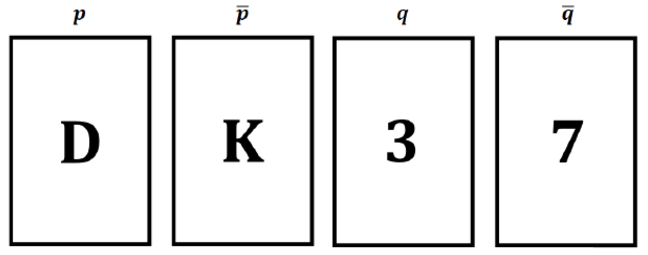
\includegraphics[scale=0.5]{wasonAbstract}
\caption{The Abstract case of the Wason Selection Task}
\end{center}
\label{fig:wst}
\end{figure}

The Abstract case of the WST presents the subject with four cards on a table as shown in Figure~\ref{fig:wst}. Their face-up sides read $D, K, 3,$ and $7$. Participants are told that each card has a number on one side and a letter on the other. They are then asked which cards must be turned over to test the rule:

\begin{center}
``If there is a $D$ on one side of the card, then the other side shows $3$."
\end{center} 

\begin{table}
\begin{center}


\begin{tabular}{ c c c}
  \textbf{$D$}&  \textbf{$3$}& \textbf{$3\leftarrow D$} \\ 
 $\top$ & $\top$ & $\top$\\  
 $\top$ & $\bot$ & $\bot$\\  
 $\bot$ & $\top$ & $\top$\\
 $\bot$ & $\bot$ & $\top$
\end{tabular}
\caption{Propositional evaluation of the conditional $3 \leftarrow D$ for each possible truth value of $3$ and $D$.}
\label{tbl:wst_classical}
\end{center}
\end{table}


This task requires the participants to find possible defeaters for the conditional rule. Assuming $\textrm{``if } \phi \textrm{ then }\psi \textrm{"} \leftrightarrow (\psi \leftarrow \phi)$, Table~\ref{tbl:wst_classical} shows that the cards $D$ and $7$ (i.e. $\lnot 3)$ are both possible defeaters to the rule $3\leftarrow D$ because the rule $3 \leftarrow D$ is only falsified when the interpretation maps $(D,\top)$ and $(3, \bot)$ and so any observed card which allows a possible world with both of those assignments is a possible defeater. If a participant were to turn the $D$ card and find a number that was not $3$, or were to a turn the card $7$ and find the letter $D$ on the other side, the conditional would not hold. Thus these two cards must be turned to check the rule. However, human subjects very seldom choose this classical answer set and instead overwhelmingly prefer to turn the cards $D$ and $3$. Table~\ref{tbl:can} shows the most common card selection sets for participants.

A great many cognitive theories have been applied to these results, with varying degrees of success \cite{ragni2017formal}. This paper will focus on the WCS interpretation of the task provided by \citep{ragni2017wason}. This approach assumed an initial knowledge base $\textit{KB}$ containing only the conditional $(3|D)$ and an interpretation of the conditional as follows:

\begin{itemize}
\item $I_\textrm{\L}(\psi|\phi)\leftrightarrow I_\textrm{\L}(\psi \leftarrow \phi \land \lnot \textit{ab})$, where $I_\textrm{\L}$ denotes the interpretation of the conditional under 3-valued @TODOLukaname logic, and \textit{ab} represents a license for implication. @TODOmovetoprelimsection
\end{itemize}

@TODOrefdietsholldobler showed that the abstract case of the WST could be modelled using the WCS and 3-valued @lucasciewics logic. Using the conditional as the initial logic program, we write $KB=(S=\{\},\Delta=(3|D))$. Treating conditionals as licenses for implication $KB$ can be rewritten as $KB=(3\leftarrow D \land \lnot ab)$ where $ab$ is an abnormality predicate. Now $\textrm{lm wc}(KB)=\{\}\{ab\}$, and no information is obtained that could either verify or falsify the conditional. In order to adapt the WCS to the WST @TODOname introduced the concept of observation support.

The set of abducibles $A$ corresponds to positive and negative facts which are not assigned in $KB$. For the WST as formulated here $A=\{D\leftarrow \top,D\leftarrow \bot,3\leftarrow \top,3\leftarrow \bot,K\leftarrow \top,K\leftarrow \bot,7\leftarrow \top,7\leftarrow \bot\}$.
 An observation $O$ is explained by a minimal explanation $\epsilon \in A$ if and only if $O$ holds in $\textrm{lm wc}(KB\cup\epsilon)$. Table~@TODOfig shows the least models that can be drawn for the observations $D$, $3$, $K$, and $7$. If a least model obtained in this way contains atoms and atomic assignments that could invalidate the conditional (i.e. make $I_{\textrm{lm wc}(KB\cup \epsilon)}(3\leftarrow D \land ab)\models \bot$), then the observed card should be turned. Figure~@TODOref shows the derivation of $\textrm{lm wc}(KB\cup \epsilon)$ for $\epsilon=D, \epsilon=3, \epsilon=K$, and $\epsilon=7$ @TODOchangetextinfiguretosayetainsteadofobservation.


This simple interpretation of the WST which applies abduction to the initial knowledge base to derive observation is sufficient to model the general reasoner. It does not however explain any of the other deviant cases which are observed in Table~\ref{tbl:can}. Why, for example, should it be considered accurate if it gives no information about the classically accurate choice of the $D$ and $7$ cards, chosen by 19 participants, a significant portion? Instead, consider how these aberrant reasoners could be modelled. Perhaps they use extra computational steps or omit steps? This author has previously shown that the WCS is able to model these individual reasoners \citep{breu2019weak}\footnote{My contribution to this paper was the initial proposal of the extensions, their integration, the silencing mechanism used for modelling individual reasoners, and the broad idea of the stochastic evaluation technique itself.} by including three simple processes: basic weak completion, abduction as we have already discussed in this section, and contraposition. By including these three processes, and stochastically controlling when they are activated or silenced, it has been shown that not only is this extended framework able to model the major cases of the WCS, but very close approximations to empirical results can also be drawn.

\subsubsection*{Basic Weak Completion}
\begin{figure}
\centering 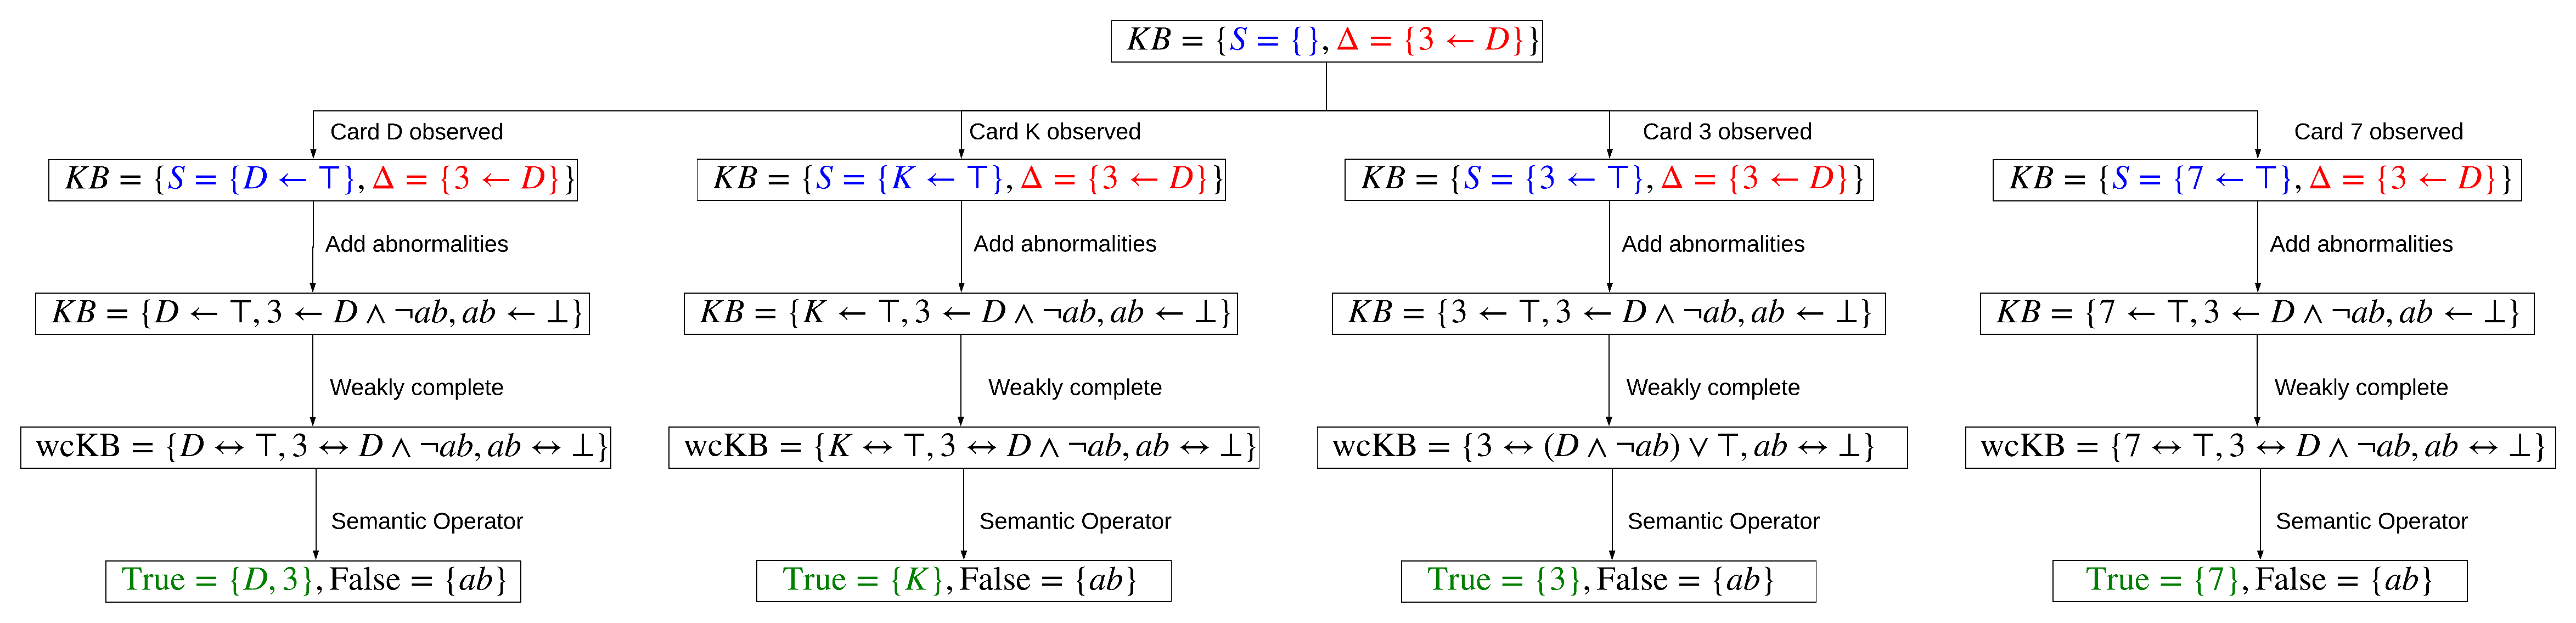
\includegraphics[scale=0.4]{WST_WCS}
\caption{Application of the WCS to the abstract case of the WST for the basic weak completion approach.}
\label{wst_wcs}
\end{figure}
Basic weak completion ignores the existence of other least models which may validate the inference $(3|D)$ and, instead handles only those cases where $\epsilon \leftrightarrow (O\leftarrow \top)$. That is, only information about the currently observed card is considered in the abductive framework. Figure~\ref{wst_wcs} illustrates this process for each of the four observations: $D$, $3$, $K$, and $7$. Now only $\textrm{wc lm}(KB \cup (D \leftarrow \top))$ now provides assignments which could invalidate the inference if they were otherwise. Observing the card $3$ no longer leads to the decision to turn the card because only the case $\epsilon = (3\leftarrow \top)$ is considered and the case $\epsilon = (D \leftarrow \top)$ is not considered.

\subsubsection*{Contraposition}
\begin{table}
\begin{center}
\begin{tabular}{ c c c }
 \textbf{Iteration} & \textbf{$\top$} & \textbf{$\bot$} \\ 
 0 &  &  \\  
 1 &  $7$ & $ab_1$, $ab_2$  \\  
 2 &  $7$ & $3$, $ab_1$, $ab_2$  \\
 3 &  $7$, $D'$ & $3$, $ab_1$, $ab_2$  \\
 4 &  $7$, $D'$ & $3$, $ab_1$, $ab_2$, $D$  
\end{tabular}
\caption{Applying the Weak Completion Semantics and Contraposition to the $7$ card of the WST.}
\label{tbl:7cont}
\end{center}
\end{table}

Contraposition explicitly makes use of \textit{modus tolens}, usually assumed to be silenced in human cognition to derive certain canonical cases in the WST. Using contraposition it becomes possible to model individual participants who choose to turn the cards $D$ and $7$ (the classical response).

@TODO change
Contraposition is applied as follows for the initial knowledge base $KB$:
\begin{enumerate}
\item For each conditional $(\psi|\phi)\in KB'$ :
\begin{itemize}
\item Add the conditional $(\phi'|X)$ to $\Delta$, where $X$ is the other possible value for that card face\footnote{$(D,K),(3,7)$}.
\item Add the fact $\phi\leftarrow \lnot \phi'$ to $S$.
\end{itemize}
\item Interpret conditionals as licenses for implication.
\item Apply the WCS as normal.
\end{enumerate}

Using this technique, and applying basic weak completion (i.e. only considering the case $\epsilon\leftrightarrow(O\leftarrow \top)$ it is possible to model the classical case of the WST. The resolution for the $7$ card is as follows:

\[
KB = (S=\{\},\Delta=\{(3|D)\})
\]
\[
KB' = (S=\{D \leftarrow  \lnot D'\},\Delta\{=(3|D),(D'|7)\})
\]
\[
KB' = \{3 \leftarrow D \land \lnot \text{ab}_1, D' \leftarrow 7 \land \lnot \text{ab}_2, \text{ab}_1 \leftarrow \bot, \text{ab}_2 \leftarrow \bot\}\}
\]
\[
KB'\cup (7\leftarrow\top) = \{3 \leftarrow D \land \lnot \text{ab}_1, D' \leftarrow 7 \land \lnot \text{ab}_2, \text{ab}_1 \leftarrow \bot, \text{ab}_2 \leftarrow \bot, 7 \leftarrow \top\}\}
\]

\[
\text{wc}KB'\cup (7\leftarrow\top) = \{3 \leftrightarrow D \land \lnot \text{ab}_1, D' \leftrightarrow 7 \land \lnot \text{ab}_2, \text{ab}_1 \leftrightarrow \bot, \text{ab}_2 \leftrightarrow \bot, 7 \leftrightarrow \top\}\}
\]
\begin{equation} \label{eqn:wst_contra}
\textrm{wc} (KB'\cup (7\leftarrow\top)) = \{3 \leftrightarrow D \land \lnot ab_1, D' \leftrightarrow (\lnot 3 \land ab_2) \lor (\lnot D),  ab_2\leftrightarrow \bot, ab_1\leftrightarrow \bot, 7\leftrightarrow\top \}
\end{equation}

Table~\ref{tbl:7cont} shows the computation of $\textrm{lm wc} (KB'\cup (7\leftarrow\top))$. From this, it is possible to deduce that the card $7$ must be turned. Figure~\ref{fig:wstcano} illustrates the use of these extensions to derive all four of the canonical cases of the WST.

\subsubsection*{Combined Model}
By combining our contraposition and adductive rules for inferences which were discussed in \citep{dietz2012computational}'s paper, it is possible to model the case where the cards $D$, $K$, and $7$ are turned (Figure~\ref{wstcano} @TODOfigures?).

This work showed that all canonical cases of the weak completion semantics could be modelled by activating or silencing these three processes on the initial knowledge base. The intuition that a discrete and systematic succession of well-founded processes could be used to model multiple different results for the same experiment was the inspiration for the SCP framework which this thesis introduces.


\begin{figure}
\centering \includegraphics[scale=.6]{wstcano}
\caption{Using the abduction and contraposition extensions to derive all four canonical cases. @TODOredoWithCards}
\label{fig:wstcano}
\end{figure}








\section{More}